
\def\anon{1} %% set to 1 for anonymous submissions, hides acknowledgements and author names
\def\full{1} %% set to 0 for springer proceedings


\ifnum\full=1
\documentclass[11pt]{llncs}


\addtolength{\parskip}{1pt}
\else
\documentclass[10pt, runningheads]{llncs}
\usepackage{times}

\fi




\usepackage{makeidx}
\usepackage[dvips]{graphicx}
\usepackage{graphicx}

\usepackage{comment}

\usepackage{listings}
\usepackage[mathscr]{eucal}
\usepackage{bm}
\usepackage{array}
\usepackage{url}
\usepackage{calc}
\usepackage{float}
\usepackage{latexsym}
\usepackage{rotating}
\DeclareGraphicsExtensions{.eps,.jpg,.png,.pdf}
%\usepackage[usenames, dvipsnames]{xcolor}
\usepackage[dvipsnames]{xcolor}
\usepackage[sort,nocompress]{cite}
\usepackage{colortbl}
\usepackage{multirow}
\usepackage{lscape}
\usepackage{amsmath}
\let\proof\relax
\let\endproof\relax
\usepackage{amsthm,amsfonts,amssymb}
\usepackage{hyperref}
\usepackage{pdflscape}


%\usepackage{natbib}

\def\rmdefault{ptm}

\usepackage{setspace}
\usepackage{color}
\ifnum\full=1
\usepackage[margin=0.9in]{geometry}
\usepackage{fullpage}

\setlength{\parskip}{0cm}

%\setstretch{1.03}
%\addtolength{\parskip}{1pt}
\setcounter{page}{0}
\renewcommand{\tabcolsep}{5pt}
\else
\renewcommand{\tabcolsep}{0pt}
\fi

\renewcommand{\arraystretch}{1.2}

\hyphenpenalty=5000
\tolerance=1000




%\ifnum\full=1
%\usepackage{natbib}
%\bibliographystyle{alpha}
%\setlength{\bibsep}{0pt}
%\renewcommand{\bibsection}{\section*{References}\small}
%\else
%\usepackage[numbers]{natbib}
%\bibliographystyle{splncs04}
%\fi



\DeclareMathOperator{\Exp}{E}
\DeclareMathOperator{\Var}{Var}
\DeclareMathOperator{\poly}{poly}
\DeclareMathOperator{\Supp}{Supp}

\usepackage{enumitem}


\usepackage{tikz}
\usetikzlibrary{arrows,shapes}
\usetikzlibrary{plotmarks}


%notes

%\definecolor{myorange}{rgb}{0.99,0.6,0.25}
%\newcommand{\pmnote}[1]{\colorbox{myorange}{\parbox{0.9\linewidth}{[{\footnotesize {\bf PM:} { {#1}}}]}}}


\definecolor{mycolor}{rgb}{0.75,0.95,0.05}
\newcommand{\pmnote}[1]{\colorbox{mycolor}{\parbox{0.9\linewidth}{[{\footnotesize {\bf PM:} { {#1}}}]}}}

\newcommand{\tsnote}[1]{\colorbox{orange}{\footnotesize\color{white}\textbf{TS: }#1}}

\definecolor{unmellowyellow}{rgb}{1.0, 1.0, 0.4}
\newcommand{\agnote}[1]{\colorbox{unmellowyellow}{\parbox{0.9\linewidth}{[{\footnotesize {\bf AG:} { {#1}}}]}}}
%% Sets

\newcommand{\Z}{\mathbb{Z}}
\newcommand{\N}{\mathbb{N}}
\newcommand{\R}{\mathbb{R}}
\newcommand{\C}{\mathbb{C}}
\newcommand{\F}{\mathbb{F}}
\newcommand{\Znm}{\mathbb{Z}_q^{n \times m}}

%matrices
\newcommand{\matzero}{\mathbf{0}}
\newcommand{\matA}{\mathbf{A}}
\newcommand{\matB}{\mathbf{B}}
\newcommand{\matC}{\mathbf{C}}
\newcommand{\matE}{\mathbf{E}}
\newcommand{\matF}{\mathbf{F}}
\newcommand{\matG}{\mathbf{G}}
\newcommand{\matI}{\mathbf{I}}
\newcommand{\matM}{\mathbf{M}}
\newcommand{\matP}{\mathbf{P}}
\newcommand{\matR}{\mathbf{R}}
\newcommand{\matS}{\mathbf{S}}
\newcommand{\matT}{\mathbf{T}}
\newcommand{\matU}{\mathbf{U}}
\newcommand{\matV}{\mathbf{V}}
\newcommand{\matW}{\mathbf{W}}
\newcommand{\matX}{\mathbf{X}}
\newcommand{\matY}{\mathbf{Y}}
\newcommand{\matZ}{\mathbf{Z}}


%vectors
\newcommand{\veca}{\mathbf{a}}
\newcommand{\vecb}{\mathbf{b}}
\newcommand{\vecc}{\mathbf{c}}
\newcommand{\vecd}{\mathbf{d}}
\newcommand{\vece}{\mathbf{e}}
\newcommand{\veci}{\mathbf{i}}
\newcommand{\vecj}{\mathbf{j}}
\newcommand{\veck}{\mathbf{k}}
\newcommand{\vecl}{\mathbf{l}}
\newcommand{\vecm}{\mathbf{m}}
\newcommand{\vecp}{\mathbf{p}}
\newcommand{\vecr}{\mathbf{r}}
\newcommand{\vecs}{\mathbf{s}}
\newcommand{\vecv}{\mathbf{v}}
\newcommand{\vecw}{\mathbf{w}}
\newcommand{\vecu}{\mathbf{u}}
\newcommand{\vecx}{\mathbf{x}}
\newcommand{\vecy}{\mathbf{y}}
\newcommand{\vecz}{\mathbf{z}}





%FiLIP notations

\newcommand{\FLIP}{\textsf{FLIP}}
\newcommand{\IFPl}{\text{Improved Filter Permutator} }
\newcommand{\IFPs}{\text{IFP} }

\newcommand{\FiLIP}{\textsf{FiLIP}}
\newcommand{\FiLIPDSM}{\mathsf{FiLIP}_{\mathsf{DSM}}}
\newcommand{\FiLIPXMAJ}{\mathsf{FiLIP}_{\mathsf{XMAJ}}}

%Boolean functions

\newcommand{\Bfn}[1]{\mathcal{B}_{#1}}
\newcommand{\BN}{\mathcal{B}_n}
\newcommand{\Bn}[1]{\mathcal{B}_{#1}}
\newcommand{\Bnstar}[1]{\mathcal{B}_{#1}^*}

\newcommand{\Bvad}[3]{\mathcal{B}({#1},{#2},{#3})}


\newcommand{\AI}{\mathsf{AI}}
\newcommand{\AN}{\mathsf{AN}}
%\newcommand{\difAN}[1]{\Delta_{\mathsf{AN}}(#1)}
%\newcommand{\DAN}{\mathsf{d}\mathsf{AN}}
%\newcommand{\Sd}{\mathsf{S}_\mathsf{d}}
\newcommand{\SD}{\mathsf{SD}}
\newcommand{\FAI}{\mathsf{FAI}}
\newcommand{\NL}{\mathsf{NL}}
\newcommand{\NLk}[1]{\mathsf{NL}_{#1}}
%\newcommand{\NLd}{\mathsf{NL_d}}
\newcommand{\res}{\mathsf{res}}
\newcommand{\bal}{\mathsf{bal}}
\newcommand{\gnlk}{\mathsf{GWNL}}


\newcommand{\DS}[1]{\mathsf{DS}(#1)}
\newcommand{\DSR}[2]{\mathsf{DS}^{#2}(#1)}
%\newcommand{\matAI}[3]{\mathbf{A}_{#2,#3}(#1)}

\newcommand{\WPB}[1]{\mathcal{WPB}_{#1}}
\newcommand{\WAPB}[1]{\mathcal{WAPB}_{#1}}
\newcommand{\SWAPB}[1]{\mathcal{SWAPB}_{#1}}
\newcommand{\SYM}[1]{\mathcal{SYM}_{#1}}
%for affine weightwise: degree and number of variables
\newcommand{\WD}[2]{\mathcal{WD}^{#1}_{#2}}
\newcommand{\Ekn}[2]{\mathsf{E}_{#1,#2}}
\newcommand{\Code}[2]{\mathsf{P}_{#1,#2}}
\newcommand{\mdist}[2]{\mathsf{d}_{#1,#2}}
%\newcommand{\Dka}[2]{\mathsf{D}_{#1}(#2)}
\newcommand{\Dnka}[3]{\mathsf{D}_{#1,#2}(#3)}

\newcommand{\dis}{\mathsf{c_1}}




\newcommand{\mnlk}[2]{\mu_{#1,#2}}
\newcommand{\Mnlk}[2]{\mathsf{M}_{#1,#2}}
\newcommand{\mnl}[1]{\mu_{#1}}
\newcommand{\Mnl}[1]{\mathsf{M}_{#1}}

\newcommand{\DistWkn}[2]{\mathfrak{W}_{#1,#2}}
\newcommand{\DistWn}[1]{\mathfrak{W}_{#1}}
\newcommand{\Dkn}[2]{\mathfrak{D}_{#1,#2}}
\newcommand{\Dn}[1]{\mathfrak{D}_{#1}}

\newcommand{\kraw}[3]{\mathsf{K}_{#1}(#2,#3)}
\newcommand{\phikn}[2]{\varphi_{#1,#2}}

\newcommand{\const}[2]{g_{#1,#2}}
\newcommand{\setn}[1]{S_{#1}}
\newcommand{\symsetsmall}[1]{A_{#1}}
\newcommand{\symset}[2]{B_{#1,#2}}


%usual notations
\newcommand{\supp}{\mathsf{supp}}
\newcommand{\suppk}[1]{\mathsf{supp}_{#1}}
\newcommand{\w}{\mathsf{w_H}}
\newcommand{\hd}{\mathsf{d_H}}
\newcommand{\degg}{\mathsf{deg}}
\newcommand{\Span}{\mathsf{Span}}
\newcommand{\rank}{\mathsf{rank}}
%Walsh transform
\newcommand{\wt}[1]{\mathcal W_{#1}} 
\newcommand{\Wsupp}[1]{\mathsf{Wsupp}_{#1}} 
%restricted Walsh transform W_k,a (f)
\newcommand{\wtk}[2]{\mathcal{W}_{#1,#2}} 

%S-equivalent classes
\newcommand{\sclass}[1]{\mathcal{S}(#1)}


\newcommand{\set}[1]{\left\{#1\right\}}
\newcommand{\mAN}[1]{\mathsf{d}_{#1}}


%gates
\newcommand{\AND}{\textsf{AND}}
\newcommand{\XOR}{\textsf{XOR}}
\newcommand{\MUX}{\textsf{MUX}}


%families of functions
\newcommand{\MAJ}{\textsf{MAJ}}
\newcommand{\DSM}{\textsf{DSM}}
\newcommand{\XORTHR}{\textsf{XOR-THR}}
\newcommand{\XORMAJ}{\textsf{XOR-MAJ}}

\newcommand{\xorlk}[2]{{\mathsf{XOR}}_{#1}  \mathsf{M}_{#2}} 
\newcommand{\xormaj}[2]{{\mathsf{XOR}}_{#1}  \mathsf{MAJ}_{#2}} 
%\newcommand{\xorthr}[3]{{\mathsf{XOR}}_{#1}  \mathsf{T}_{{#2},{#3}}} 
\newcommand{\xorthr}[3]{{\mathsf{XOR}}_{#1}+\mathsf{T}_{{#2},{#3}}}
\newcommand{\tri}[1]{{T}_{#1}}
\newcommand{\thr}[2]{\mathsf{T}_{{#1},{#2}}}
\newcommand{\xor}[1]{\mathsf{XOR}_{#1}}
\newcommand{\maj}[1]{\mathsf{MAJ}_{#1}}


\newcommand{\nbf}[1]{\mathsf{C}_{#1}}
\newcommand{\nbfodd}[2]{\mathsf{A}_{#1,#2}}
\newcommand{\nbfeven}[2]{\mathsf{B}_{#1,#2}}

%direct sum vector and simplified value vector
\newcommand{\dsv}[1]{\mathbf{m}_{#1}}
\newcommand{\svv}[1]{\mathbf{s}_{#1}}

% Define a custom theorem style for bold optional arguments
\newtheoremstyle{boldoptional} % Name of the style
  {3pt}                        % Space above
  {3pt}                        % Space below
  {\itshape}                   % Body font
  {}                           % Indent amount
  {\bfseries}                  % Theorem head font
  {.}                          % Punctuation after theorem head
  { }                          % Space after theorem head
  {\thmname{#1}\thmnumber{ #2}\thmnote{ (\textbf{#3})}} % Bold optional argument

% Apply the new style to Property
\theoremstyle{boldoptional}
\newtheorem{Prop}{Property}
\newtheorem{Cons}{Construction}


% For algorithms
\usepackage{algorithm,algpseudocode}

\renewcommand{\algorithmicrequire}{\textbf{Input:}}
\renewcommand{\algorithmicensure}{\textbf{Output:}}
% \renewcommand{\ALG@name}{Construction}
\newenvironment{constr}[1][htb]{%
\floatname{algorithm}{Construction}% Update algorithm name
   \begin{algorithm}[#1]%
  }{\end{algorithm}}
 
\algnewcommand\algorithmicparfor{\textbf{par-for}}
\algdef{S}[FOR]{ParFor}[1]{\algorithmicparfor\ #1\ \algorithmicdo}
 
%latin

\newcommand{\ie}{\textit{i.e.}}
\newcommand{\eg}{\textit{e.g.}}
\newcommand{\ea}{\textit{et al.}}

%Tim's stuff
\newtheorem{Corollary}{Corollary}
\newcommand{\ii}{\mathrm i\mkern1mu} %Imaginary unit
\newcommand{\ee}{\mathrm e\mkern1mu} %Euler constant
\newcommand{\dd}{\,\mathrm d} %Differential
\newcommand{\ui}[1]{^{(#1)}} %Upper index
\newcommand{\mycomment}[1]{} %Comment out entire parts
\usepackage{mleftright}
\mleftright %Less space when using \left and \right


\newcommand{\tablecaption}[1]{%
   \vspace{3pt} % Adds space above the caption
   \caption{#1} % Displays the caption text
}

\let\leq=\leqslant %Replace symbol for \leq
\let\geq=\geqslant %Replace symbol for \geq

\newcommand{\hwbf}{\textsf{HWBF}}

%No line break before lists
\makeatletter
\@beginparpenalty=10000
\makeatother


\begin{document}
	\title{Draft: Notes on the revised Hidden weight function}

	
	\titlerunning{Notes on the revised Hidden weight function}
	\author{
		\mbox{Pierrick M\'eaux}\inst{1}
	}
	
	\authorrunning{ P. M\'eaux}
	
	\institute{
	Luxembourg university, Luxembourg\\
		\email{pierrick.meaux@uni.lu}		
	}
	

	
	
	
	%----------------------------------------------------------------
	\maketitle


\institute{
	University of Luxembourg, Luxembourg\\
	\email{pierrick.meaux@uni.lu}		
}	
	
	\begin{abstract}
	
		
	\end{abstract}


\section{Introduction}

\section{Preliminaries}


\subsection{Boolean functions and weightwise considerations}

In this part we recall general concepts on Boolean functions and their weightwise properties we use in this article. 
For a deeper introduction on Boolean functions and their cryptographic parameters we refer to the survey of \eg~\cite{Carlet20} and to~\cite{TOSC:CarMeaRot17} for the weightwise properties, also called properties on the slices.
For $k \in [0,n]$ we denote $\Ekn{k}{n}$ the set $\{x\in \F_2^n \, | \, \w(x)=k  \}$ and call it slice of the Boolean hypercube (of dimension $n$). 
Accordingly, the Boolean hypercube is partitioned into $n+1$ slices where the elements have the same Hamming weight.

\begin{definition}[Boolean Function]\label{def:bool_f}
	A Boolean function $f$ in $n$ variables is a function from $\F_2^n$ to $\F_2$. 
	The set of all Boolean functions in $n$ variables is denoted by $\BN$, and we denote $\BN^*$ the set without the null function.
\end{definition}


To denote when a property or a definition is restricted to a slice we use the subscript $k$. 
For example, for a $n$-variable Boolean function $f$ we denote its support $\supp(f)=\{x\in \F_2^n \, | \, f(x)=1  \}$ and we denote $\suppk{k}(f)$ its support restricted to a slice, that is $\supp(f)\cap \Ekn{k}{n}$.


\begin{definition}[Balancedness]\label{def:balancedness}
	A Boolean function $f\in \BN$ is called balanced if $|\supp(f)|=2^{n-1}=|\supp(f+1)|$. 
	
	For $k\in [0,n]$ the function is said balanced on the slice $k$ if $||\suppk{k}(f)|-|\suppk{k}(f+1)| |\le 1$. In particular when $|\Ekn{k}{n}|$ is even $|\suppk{k}(f)|=|\suppk{k}(f+1)|=|\Ekn{k}{n}|/2$.
\end{definition}

\begin{definition}[Algebraic Normal Form (ANF) and degree]\label{def:anf}
	We call Algebraic Normal Form of a Boolean function $f$ its $n$-variable polynomial representation over $\F_2$ (\textit{i.e.} belonging to $\F_2[x_1,\dots,x_n]/(x_1^2+x_1,\dots,x_n^2+x_n)$):
	\[f(x_1,\dots,x_n)= \sum_{I \subseteq [1,n]} a_I \left( \prod_{i \in I} x_i \right) \]%x_1,\dots,x_n=\sum_{I \subseteq [1,n]} a_I x^I,\]
	where $a_I\in \F_2$. 	
	The (algebraic) degree of $f$, denoted $\degg(f)$ is: \[\degg(f)=\
	\max_{I\subseteq [1,n]}\{ |I|\, | \, a_I=1\}  \text{ if $f$ is not null},0  \text{ otherwise}.\]
\end{definition}




\begin{definition}[Walsh transform and restricted Walsh transform]\label{def:walsh_transform}
	Let $f\in \Bn{n}$ be a Boolean function, its Walsh transform $\wt{f}$ at $a \in \F_2^n$ is defined as:
	\[  \wt{f} (a) := \sum_{x \in \F_2^n} (-1)^{f(x) +  a \cdot x }.\]
	%	The Walsh support is the set $\Wsupp{f}:=\{ a\in \F_2^n\, | \, \wt{f} (a) \neq 0 \}$.
	Let $f\in \Bn{n}$, $S \subset \F_2^n$, its Walsh transform restricted to $S$ at $a \in \F_2^n$ is defined as:
	\[  \wt{f,S} (a) := \sum_{x\in S} (-1)^{f(x)+ax}.\]
	For $S=\Ekn{k}{n}$ we denote $\wt{f,\Ekn{k}{n}} (a)$ by $\wtk{f}{k}(a)$.%, and for $a= 0_{n}$ we denote $\wtk{f}{k}(a)$ as $\wtk{f}{k}(0)$.
\end{definition}


	


%\begin{definition}[Algebraic Immunity] \label{def:ai}
%	The algebraic immunity of a Boolean function $f\in \Bfn{n}$, denoted as $\AI(f)$, is defined as:
%	\[ \AI(f) = \min_{g \neq 0}\{ \degg(g) \; | \; fg = 0 \; \text{or} \; (f + 1)g = 0 \}{,} \]
%	where $\degg(g)$ is the algebraic degree of $g$.
%	The function $g$ is called an annihilator of $f$ (or $f + 1$). 
%	Additionally we denote $\AN(f) = \min_{g \neq 0}\{ \degg(g) \; | \; fg = 0\}$.
%\end{definition}

\begin{Prop}[Nonlinearity on the slice, adapted from~\cite{TOSC:CarMeaRot17}, Proposition 6]\label{prop:nlk}
	Let $n\in \N^*, k\in [0,n]$, for every $n$-variable Boolean function $f$ over $\Ekn{k}{n}$:
	\[ \NLk{k}(f)=\frac{|\Ekn{k}{n}|}{2} -\frac{\max_{a\in \F_2^n} |\wtk{f}{k}(a)|}{2}  .\]
\end{Prop}


\subsection{Symmetric Functions}


The $n$-variable \emph{Boolean symmetric functions} are those that are constant on each slice $\Ekn{k}{n}$ for $k\in [0,n]$. 
This class has been assiduously studied in the context of cryptography, see \eg \cite{IEEE:Carlet04,IEEE:CanVid05,INDO:BraPre05,DM:SarMai07,IEEE:QFLW09,CCDS:Meaux21,IEEE:CarMea21}.
In this paper we mainly consider two families of symmetric functions, which are both bases of the symmetric functions:

\begin{definition}[Elementary symmetric functions]
Let $i\in [0,n]$, the elementary symmetric function of degree $i$ in $n$ variables, denoted $\sigma_{i,n}$, is the function which ANF contains all monomials of degree $i$ and no monomials of other degrees. 
\end{definition}
\begin{definition}[Slice indicator functions]
 Let $k\in [0,n]$, the indicator function of the slice of weight $k$ is defined as:
 \[\forall  x\in \mathbb{F}_2^{n}, \quad \phikn{k}{n}(x) = 1 \text{ if and only if } \w(x) = k.\]
\end{definition}
We recall that bent functions are those Boolean functions achieving maximal nonlinearity.



\begin{Prop}[Weightwise restricted Walsh transform and addition of symmetric function (~\cite{INDO:GinMea22}, Proposition $4$)]\label{prop:AddSym}
	Let $n\in \N^*$, $k\in [0,n]$ and $f \in \Bn{n}$, the following holds on $f+\phikn{k}{n}$
	\[\forall a\in \F_2^n, \forall i\in [0,n]\setminus \{k\}, \wtk{f+\phikn{k}{n}}{i}(a)=\wtk{f}{i}(a),\text{ and } \wtk{f+\phikn{k}{n}}{k}(a)=-\wtk{f}{i}(a).\]	
\end{Prop}












\section{Main section}
%\subsection{Restricted Walsh transform of $f$ in a recursive fashion}

We study the function $f$ in an even number of variables $n$ defined as the following:
\[f(x_1,\cdots,x_n)=\left(\sum_{i=1}^{n/2} (x_i+1) x_{i+\frac{n}{2}}\right) + \sum_{k=0}^n \phikn{k}{n} x_k.\]

We study the restricted Walsh transform  of $f$ to bound its nonlinearity.

\begin{align*}
\wtk{f}{k}(a)&=\sum_{x \in \Ekn{k}{n}} (-1)^{f(x)+ax}\\
&=\sum_{x \in \Ekn{k}{n}} (-1)^{x_k + \sum_{i=1}^{n/2} (x_i+1) x_{i+\frac{n}{2}}+ ax}\\
&=\sum_{x \in \Ekn{k}{n}} (-1)^{\sum_{i=1}^{n/2} x_i x_{i+\frac{n}{2}}+ (c)x},
\end{align*}
where $c$ is the $n$-length binary vector such that $c=a+e_k+\sum_{i=n/2+1}^n e_i$ where the $e_i$ denotes the canonical vector with "1" in position $i$.

Accordingly, we can study the restricted Walsh transform of this function by analyzing the one of $\sum_{i=1}^{n/2} x_i x_{i+\frac{n}{2}}$, for all $a$. We introduce the following notations.

\begin{definition}
Let $n\in \N$ be an even number, and $a\in \F_2^n$. We denote $d_n$ the function given by: $d_n(x)=\sum_{i \text{ odd}}^n x_i x_{i+1}$, 
and we denote by $\Dnka{n}{k}{a}$:
\[\Dnka{n}{k}{a}= \sum_{x\in \Ekn{k}{n}} (-1)^{d_n(x) +a x}\]
\end{definition}
The limit case of $n=0$ yields that $\Dnka 0ka=1$ if $k=0$ and $\Dnka 0ka=0$ otherwise.

With these notations we obtain a recursive relation for $\Dnka{n}{k}{a}$, and therefore for $\wtk{f}{k}(a)$, denoting $b=(a_1,\cdots,a_{n-2})$ and $y=(x_1,\cdots,x_{n-2})$, we get for any even $n\geq 2$:

\begin{align*}
\Dnka{n}{k}{a}&=\sum_{x\in \Ekn{k}{n}} (-1)^{d_n(x) +a x}\\
&=\sum_{x\in \Ekn{k}{n-2}} (-1)^{d_{n-2}(y) +b y}+
\sum_{x\in \Ekn{k-1}{n-2}} (-1)^{d_{n-2}(y) +b y + a_{n-1}}\\
&+\sum_{x\in \Ekn{k-1}{n-2}} (-1)^{d_{n-2}(y) +b y + a_{n}}
+\sum_{x\in \Ekn{k-2}{n-2}} (-1)^{d_{n-2}(y) +b y +1 + a_{n-1}+ a_{n}}\\
&=\Dnka{n-2}{k}{b}+\left((-1)^{a_{n-1}} + (-1)^{a_{n}}\right)\Dnka{n-2}{k-1}{b} + (-1)^{1+a_{n-1}+a_n} \Dnka{n-2}{k-2}{b}.
\end{align*}

Then it gives three cases:
\begin{itemize}
	\item if $a_{n-1}=a_n=0$, then $\Dnka{n}{k}{a}=\Dnka{n}{k}{b}+2\Dnka{n}{k-1}{b}-\Dnka{n}{k-2}{b}$,
	\item if $a_{n-1} \ne a_n$, then $\Dnka{n}{k}{a}=\Dnka{n}{k}{b}+\Dnka{n}{k-2}{b}$,
	\item if $a_{n-1}=a_n=1$, then $\Dnka{n}{k}{a}=\Dnka{n}{k}{b}-2\Dnka{n}{k-1}{b}-\Dnka{n}{k-2}{b}$.
\end{itemize}

In this analysis we considered the different cases depending on the values of $a_{n-1}$ and $a_n$, but the same reasoning applies with any $a_i, a_{i+1}$ where $i$ is odd. 
Thereafter, the value of $\Dnka{n}{k}{a}$ depends only on the number of pairs of $a$ being $(0,0)$, $(1,1)$ or $(0,1)$ or $(1,0)$, and the values $\Dnka{2}{k}{a}$ for $k \in [0,2]$ and $a\in \{ (0,0),(1,1),(0,1)\}$.

The first values of $\Dnka{2}{k}{a}$ are listed in Table~\ref{tab:Dnka}


\begin{table}[H]
	\centering
	\begin{tabular}{|c|c|c|c|}
		\hline
		$a$ & $(0,0)$ & $(0,1)$ & $(1,1)$ \\ \hline
		$\Dnka{2}{0}{a}$ &$1$&$1$ & $1$\\ \hline
		$\Dnka{2}{1}{a}$ &$2$& $0$ & $-2$\\ \hline
		$\Dnka{2}{2}{a}$ &$-1$&$1$ & $-1$\\ \hline
	\end{tabular}
	\caption{Values of $\Dnka{2}{k}{a}$}\label{tab:Dnka}
\end{table}




The restricted Walsh transform of $f$ can the be written as \begin{align*}
\wtk{f}{k}(a)&=\sum_{x \in \Ekn{k}{n}} (-1)^{f(x)+ax}=\sum_{x \in \Ekn{k}{n}} (-1)^{\sum_{i=1}^{n/2} x_i x_{i+\frac{n}{2}}+ (c)x}\\
&=\Dnka{n}{k}{d},
\end{align*}
where $d$ is the permutation of $c$ obtained by sending the first $n/2$ elements to the odd positions, and the $n/2$ last ones to the even positions. Calling $\pi$ this permutation we can write $d=\pi(a)+ \pi(e_k)+ (0,1,0,1,\ldots,0,1)$. 
Accordingly, if $k\le n/2$, the vector $(\pi(e_k)+ (0,1,0,1,\ldots,0,1))$ has weight $n/2+1$, with one couple of consecutive elements (the first one with an odd index) being $(1,1)$ and all the others $(0,1)$. 
Otherwise,  when $k> n/2$, the vector $(\pi(e_k)+ (0,1,0,1,\ldots,0,1))$ has weight $n/2-1$, with one couple of consecutive elements (the first one with an odd index) being $(0,0)$ and all the others $(0,1)$. 

Denoting by $b$ the vector $\pi(a)+(0,1,0,1,\ldots,0,1)$, we can write the Walsh transform of $f$ in $a$ as:
\[\wt{f}(a)=\sum_{k=0}^n\Dnka{n}{k}{b+\pi(e_k)}.\]

In particular, for $a=0_n$ we can study the balancedness of $f$:
\begin{align*}
\wt{f}(0_n)&=\sum_{k=0}^n\Dnka{n}{k}{(0,1,0,1,\ldots,0,1)+\pi(e_k)}\\
&=\sum_{k=0}^{n/2}\Dnka{n}{k}{(1,1,0,1,\ldots,0,1)}+ \sum_{k=\frac{n}{2}+1}^{n}\Dnka{n}{k}{(0,0,0,1,\ldots,0,1)}
\end{align*}
Using the recursive relation we obtain:
\begin{align*}
\Dnka{n}{k}{(1,1,0,1,\ldots,0,1)}&= \Dnka{n-2}{k}{(1,1,0,1,\ldots,0,1)} + \Dnka{n-2}{k-2}{(1,1,0,1,\ldots,0,1)} \\
&=\sum_{i=0}^{n/2-1} \binom{n/2-1}{i} \Dnka{2}{k-2i}{(1,1)}\\
&=\binom{n/2-1}{k/2} \Dnka{2}{0}{(1,1)}+ \binom{n/2-1}{(k-1)/2} \Dnka{2}{1}{(1,1)}+ \binom{n/2-1}{k/2-1} \Dnka{2}{2}{(1,1)}\\
&=\binom{n/2-1}{k/2} -2 \binom{n/2-1}{(k-1)/2} - \binom{n/2-1}{k/2-1}\\
\end{align*}
Similarly, for $\Dnka{n}{k}{(0,0,0,1,\ldots,0,1)}$ we get:
\begin{align*}
\Dnka{n}{k}{(0,0,0,1,\ldots,0,1)}
%&= \Dnka{n-2}{k}{(0,0,0,1,\ldots,0,1)} + \Dnka{n-2}{k-2}{(0,0,0,1,\ldots,0,1)} \\
&=\sum_{i=0}^{n/2-1} \binom{n/2-1}{i} \Dnka{2}{k-2i}{(0,0)}\\
&=\binom{n/2-1}{k/2} \Dnka{2}{0}{(0,0)}+ \binom{n/2-1}{(k-1)/2} \Dnka{2}{1}{(0,0)}+ \binom{n/2-1}{k/2-1} \Dnka{2}{2}{(0,0)}\\
&=\binom{n/2-1}{k/2} +2 \binom{n/2-1}{(k-1)/2} - \binom{n/2-1}{k/2-1}\\
\end{align*}


%We can study the balancedness of $f$ using the $\Dnka{n}{k}{a}$ values.
Combining both we obtain:
\begin{align*}
\wt{f}(0_n)&=\sum_{k=0}^{n/2}\Dnka{n}{k}{(1,1,0,1,\ldots,0,1)}+ \sum_{k=\frac{n}{2}+1}^{n}\Dnka{n}{k}{(0,0,0,1,\ldots,0,1)}\\
&=\sum_{k=0}^{n/2} \left(\binom{n/2-1}{k/2} -2 \binom{n/2-1}{(k-1)/2} - \binom{n/2-1}{k/2-1} \right)+ \sum_{k=\frac{n}{2}+1}^{n}   \left(  \binom{n/2-1}{k/2} +2 \binom{n/2-1}{(k-1)/2} - \binom{n/2-1}{k/2-1} \right)\\
&=\sum_{k=0}^{n}\left( \binom{n/2-1}{k/2} - \binom{n/2-1}{k/2-1}\right) 
+ 2 \left( \sum_{k=\frac{n}{2}+1}^{n} \binom{n/2-1}{(k-1)/2} - \sum_{k=0}^{n/2} \binom{n/2-1}{(k-1)/2}\right)\\
&=2 \left( \sum_{k=\frac{n}{2}+1}^{n} \binom{n/2-1}{(k-1)/2} - \sum_{k=0}^{n/2} \binom{n/2-1}{(k-1)/2}\right)\\
&=2 \left( \sum_{i=\lceil n/4 \rceil}^{n/2-1} \binom {n/2-1}{i} - \sum_{i=0}^{\lfloor(n-2)/4 \rfloor} \binom{n/2-1}{i}\right).\\
\end{align*}

Then, depending on the parity of $n/2$ we obtain the the value of $\wt{f}(0_n)$ (using that $\binom{n}{k}=\binom{n}{n-k}$):
	\[\wt{f}(0_n)= \left \{
\begin{array}{l l}
0 & \text{ if } n/2 \text{ is even, } \\
-2 \binom{n/2-1}{(n-2)/4} & \text{ if }  n/2 \text{ is odd.}
\end{array}\right.\]

Accordingly, $f$ is balanced when $n=0\mod 4$ and unbalanced when $n=2 \mod 4$.

\subsection{Study of $\Dnka nka$ through Generating Functions}
For $a\in\F_2^n$, denote by $p=p(a)$ the number of odd $i\geq 1$ for which $(a_i,a_{i+1})=(0,0)$, by $q=q(a)$ the number of odd $i\geq 1$ for which $(a_i,a_{i+1})=(1,1)$, and by $r=r(a)$ the number of odd $i\geq 1$ for which $(a_i,a_{i+1})\in\{(0,1),(1,0)\}$. We then have $p+q+r=n/2$. Consider further the integer polynomial $P_a(z)$ given by the following expression:
\[
    P_a(z)=(-z^2+2z+1)^{p}\cdot(-z^2-2z+1)^{q}\cdot(z^2+1)^{r}.
\]

\begin{Prop}\label{prop:generating_fct}
    It holds that $\sum_{k\in\Z}\Dnka nka z^k= P_a(z)$.
\end{Prop}

\begin{proof}
    Proceed by induction on even $n\geq 0$. The base case $n=0$ is obvious because for $a\in\F_2^0$, we have $P_a(z)=1$, while $\Dnka 0ka=1$ if $k=0$ and $\Dnka 0ka=0$ otherwise. For the inductive step, let $n\geq 2$ be even, and assume that the corresponding formula holds for $n-2$. Using the recursive formula for $\Dnka nka$ with the notation $a=(b,a_{n-1},a_n)$, we have:
    \begin{align*}
        \begin{split}
        \sum_{k\in\Z}\Dnka nka z^k&=\sum_{k\in\Z}\Dnka{n-2}kbz^k+\big((-1)^{a_{n-1}}+(-1)^{a_{n}}\big)\sum_{k\in\Z}\Dnka{n-2}{k-1}{b}z^k\\
        &\quad+(-1)^{1+a_{n-1}+a_n}\sum_{k\in\Z}\Dnka{n-2}{k-2}{b}z^k\\
        &=P_b(z)+\big((-1)^{a_{n-1}}+(-1)^{a_{n}}\big)zP_b(z)+(-1)^{1+a_{n-1}+a_n}z^2P_b(z)\\
        &=P_b(z)\cdot\Big(z^2(-1)^{1+a_{n-1}+a_n}+z\big((-1)^{a_{n-1}}+(-1)^{a_{n}}\big)+1\Big)\\
        &=P_a(z).\qedhere
        \end{split}
    \end{align*}
\end{proof}

We can use this result to express $\Dnka n{n-k}a$  in terms of $\Dnka nka$:

\begin{Prop}\label{prop:symmetry}
    For every integer $k$, we have:
    \[
        \Dnka n{n-k}a=(-1)^{p+q+k}\Dnka nka.
    \]
\end{Prop}

\begin{proof}
    Define the degree $n$ polynomial $Q_a(z)$ in such a way that the coefficient of $z^k$ in $Q_a(z)$ is equal to the coefficient of $z^{n-k}$ in $P_a(z)$. Then we have:
    \begin{align*}
        Q_a(z)&=z^nP_a(1/z)\\
        &=(z^2+2z-1)^p\cdot(z^2-2z-1)^q\cdot(z^2+1)^r\\
        &=(-1)^{p+q}(-z^2-2z+1)^p\cdot(-z^2+2z+1)^q\cdot(z^2+1)^r\\
        &=(-1)^{p+q}P_a(-z).
    \end{align*}
    Thus the coefficient of $z^k$ in $Q_a(z)$, which is $\Dnka n{n-k}a$, is equal to the coefficient of $z^k$ in $(-1)^{p+q}P_a(-z)$, which is $(-1)^{p+q+k}\Dnka nka$.
\end{proof}

\begin{Corollary}
    If $r$ is odd, then for $k=n/2$, we have: $\Dnka n{n/2}a=0.$
\end{Corollary}

\begin{proof}
    By Property \ref{prop:symmetry}, we have $\Dnka n{n/2}a=(-1)^{p+q+n/2}\Dnka n{n/2}a=-\Dnka n{n/2}a$ because $p+q+n/2\equiv n/2-p-q\equiv r\equiv 1\bmod 2$.
\end{proof}

Another immediate case for zero coefficients is the following:
\begin{Prop}
    If $p=q$ and $k$ is odd, then $\Dnka nka=0=\Dnka n{n-k}a$.
\end{Prop}

\begin{proof}
    If $p=q$, we have $P_a(z)=(z^4-6z^2+1)^p\cdot(z^2+1)^r$, which can be seen as a polynomial in $z^2$. Thus, the coefficient $\Dnka nka$ of $z^k$ for odd $k$ must be zero in $P_a(z)$. It follows that also $\Dnka n{n-k}a=0$ by Property \ref{prop:symmetry}.
\end{proof}

\begin{remark}
    We can also use Property \ref{prop:generating_fct} to obtain $\Dnka nka$ through differentiation:
    \[
        k!\cdot\Dnka nka=\frac{\dd^k}{\dd^k z}P_a(z)\vert_{z=0}.
    \]
    Using this formula, we can for instance use a computer algebra system to deduce $\Dnka nka$ for small values of $k$, see Table \ref{tab:Dnka_small_k}. Note that even though the expression for $\Dnka n3a$ involves a division by $3$, its evaluation at specific values for $(p,q,r)$ will always yield integers. Indeed, either $p-q\equiv 0\bmod 3$, or $(p-q)^2\equiv 1\bmod 3$, in which case $2(p-q)^2+7\equiv 0\bmod 3$.
    
    \begin{table}
    	\centering
    	\begin{tabular}{|c|c|}
    		\hline
    		$k$ & $\Dnka nka$\\ \hline
    		$0$&$1$\\ \hline
            $1$&$2(p-q)$\\ \hline
            $2$&$2(p-q)^2-3(p+q)+r$\\ \hline
            $3$&$\frac 23(p-q)\left(2(p-q)^2-9(p+q)+3r+7\right)$\\ \hline
    	\end{tabular}
    	\caption{Values of $\Dnka{n}{k}{a}$ for small $k$}\label{tab:Dnka_small_k}
    \end{table}
\end{remark}

With this, we can get more cases in which $\Dnka nka=0$:

\begin{Prop}\mbox{}
    \begin{enumerate}
        \item If $n=16m$ and $\{p,q\}=\{m+\ell_s,m+\ell_{s+1}\}$ for integers $m,s\geq 0$, where $\ell_s=s(s-1)$, then $\Dnka n2a=0=\Dnka n{k-2}a$.
        \item If $n=16m+2$ and $\{p,q\}=\{m+\ell_s,m+\ell_{s+1}\}$ for integers $m,s\geq 0$, where $\ell_s=\left(6s^2+6s+(-1)^s(2s+1)-1\right)/8$, then $\Dnka n3a=0=\Dnka n{k-3}a$.
        \item If $n=16m+4$ and $\{p,q\}=\{m+\ell_s,m+\ell_{s+1}\}$ for integers $m,s\geq 0$, where $\ell_s=s^2$, then $\Dnka n2a=0=\Dnka n{k-2}a$.
        \item If $n=16m+6$ and $\{p,q\}=\{m+\ell_s,m+\ell_{s+1}\}$ for integers $m,s\geq 0$, where $\ell_s=\left(6s^2+6s-(-1)^s(2s+1)+1\right)/8$, then $\Dnka n3a=0=\Dnka n{k-3}a$.
    \end{enumerate}
\end{Prop}

\begin{proof}
    It is enough to use the expressions from Table \ref{tab:Dnka_small_k}, and replace $p$, $q$ and $r$ by their respective values. For instance, for the case $n=16m$, we replace $p$, $q$ and $r$ by $m+s(s-1)$, $m+s(s+1)$ and $6m-2s^2$ in the expression $\Dnka n2a=2(p-q)^2-3(p+q)+r$, which yields $\Dnka n2a=0$.
\end{proof}

\begin{remark}
    There are still instances where $\Dnka nka=0$ which have not been described by the above. For instance, we have $\Dnka{34}4a=0$ if $\{p,q\}=\{1,2\}$.
\end{remark}

Using Property \ref{prop:generating_fct}, we can also deduce some sums involving the $\Dnka nka$:

\begin{Prop}\mbox{}
    \begin{enumerate}
        \item The sum and alternating sum over $k$ of the $\Dnka nka$ are, respectively:
        \[
            \sum_{k=0}^n\Dnka nka=(-1)^{q}2^{n/2},\quad\sum_{k=0}^n(-1)^k\Dnka nka=(-1)^{p}2^{n/2}.
        \]
        \item The sum over the even and the odd $k$ of the the $\Dnka nka$ are, respectively:
        \[
            \sum_{k=0}^{n/2}\Dnka n{2k}a=2^{n/2-1}\big((-1)^{q}+(-1)^{p}\big),
        \]
        \[
            \sum_{k=0}^{n/2-1}\Dnka n{2k+1}a=2^{n/2-1}\big((-1)^{q}-(-1)^{p}\big).
        \]
    \end{enumerate}
\end{Prop}

\begin{proof}
    For the sum and the alternating sum, it is enough to compute $P_a(1)$ and $P_a(-1)$, respectively. The sum of the $\Dnka nka$ over the even (respectively, odd) $k$ is obtained by adding (respectively, subtracting) these two sums and dividing by $2$.
\end{proof}

One can also prove the following:

\begin{Prop}
    For a fixed integer $k\geq 1$ and sufficiently large $n\geq b(k)$, it holds that:
    \[
        \max_{a\in\F_2^n}|\Dnka nka|=|\Dnka nk{0_n}|=\left(-\frac12\right)^k\sum_{i=\lceil k/2\rceil}^{n/2}(-4)^i\binom{n/2}{i}\binom{i}{k-i}.
    \]
\end{Prop}

\begin{remark}
    In general, it also appears that the vector $a\in\F_2^n$ for which $|\Dnka nka|$ is maximal always satisfies $r(a)=0$.
\end{remark}

Also, using the Cauchy estimate on holomorphic functions, we can prove:

\begin{Prop}
    For any real number $R>0$, we have the following bound:
    \[
        |\Dnka nka|\leq\frac{(M_R)^{n/2}}{R^k},
    \]
    where $M_R$ is the maximum of $\left|z^2-2z-1\right|$ on the complex disk $|z|=R$. Explicitly, $M_R$ can be expressed as follows:
    \[
        M_R=
        \begin{cases}
            -R^2+2R+1&\text{if $R\leq\sqrt 2-1$}\\
            \sqrt 2\left(R^2+1\right)&\text{if $\sqrt 2-1\leq R\leq\sqrt 2+1$}\\
            R^2+2R-1&\text{if $R\geq\sqrt 2+1$}\\
        \end{cases}.
    \]
\end{Prop}

\begin{remark}
    Here are some interesting choices for $R$:
    \begin{itemize}
        \item Choosing $R=1/\sqrt 2$ yields that $|\Dnka nka|\leq\left(3/\sqrt 2\right)^{n/2}\cdot \sqrt 2^k$.
        \item Choosing $R=1/2$ gives $|\Dnka nka|\leq (5\sqrt 2/4)^{n/2}\cdot 2^k$.
        \item Choosing $R=1$ yields $|\Dnka nka|\leq (2\sqrt 2)^{n/2}$. This is particularly useful if $k$ is close to $n/2$.
    \end{itemize}
\end{remark}

\begin{remark}
    We can even go ahead and choose $R=R_{n,k}$ in terms of $n$ and $k$, in such a way that the upper bound of $B_{R,n,k}=(M_R)^{n/2}/R^k$ is minimized. To do this, consider any $1\leq k\leq n-1$. We can actually assume that $k\leq n/2$: if $k>n/2$, replace it by $n-k$ (recall that $|\Dnka nka|=|\Dnka n{n-k}a|$ by Property \ref{prop:symmetry}). One can show that $B_{R,n,k}$ is minimal for the following choice of $R=R_{n,k}$:
    \[
        R_{n,k}=\begin{cases}
            \frac{n-2k-\sqrt{2(n-2k)^2-n^2}}{2(n-k)}&\text{if $k\leq\frac{2-\sqrt 2}{4}\cdot n$}\\
            \sqrt{\frac{k}{n-k}}&\text{if $k\geq\frac{2-\sqrt 2}{4}\cdot n$}
        \end{cases}.
    \]
    Figure \ref{fig:cauchy_estimate} compares for $n=1\,000$ the two upper bounds we have for $|\Dnka nka|$ on a logarithmic scale: the binomial coefficient $\binom nk$ in red, and the bound $B_{R,n,k}$ with the optimally chosen $R=R_{n,k}$ in blue. The $x$-axis represents the values for $k$, while the $y$-axis represents the binary logarithm of the two bounds. In case $|k-n/2|\leq\sqrt{2}/4\cdot n$, it can be observed that the Cauchy estimate yields particularly good bounds compared to the binomial coefficients. In fact, in this case, we get:
    \[
        |\Dnka nka|\leq 2^{n/4}\sqrt{\frac{n^n}{(n-k)^{n-k}\cdot k^k}}.
    \]
    \begin{figure}
        \centering
        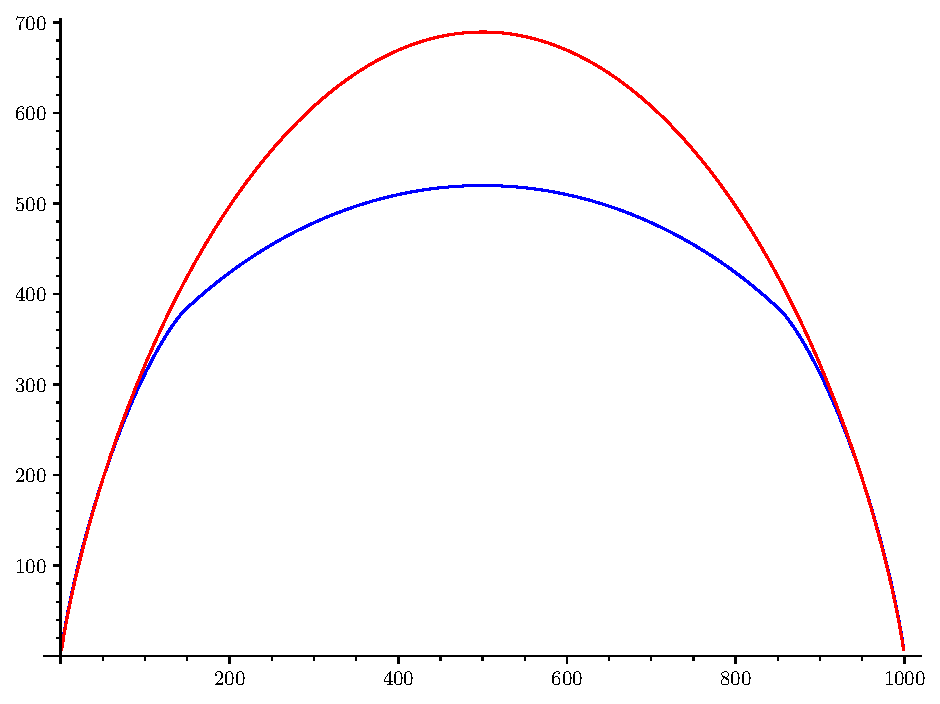
\includegraphics[width=7cm]{cauchy_estimate.pdf}
        \caption{Cauchy estimate in blue vs.\ binomial coefficients in red}
        \label{fig:cauchy_estimate}
    \end{figure}
    
    \begin{Prop}
        For every $1\leq k\leq n$, fix a Boolean vector $a\ui k\in\F_2^n$. Then we have the following bound:
        \[
            \sum_{k=1}^n\left|\Dnka nk{a\ui k}\right|\leq n\cdot 2^{3n/4}.
        \]
    \end{Prop}

    \begin{proof}
        Simply observe that $2^{n/4}\sqrt{\frac{n^n}{(n-k)^{n-k}\cdot k^k}}$ is maximal for $k=n/2$, in which case the expression reduces to $2^{3n/4}$.
    \end{proof}
\end{remark}

\newpage

%%%%%%%%%%%%%%%%%%%%%%%%%%%%%%%%%%%%%%%


\ifnum\full=0
%%%%%%%%%%%%%%%%%%%%%%%%%%%%%%%%%%%%%%%%%%%%
\bibliographystyle{splncs04}
\bibliography{add}
%%%%%%%%%%%%%%%%%%%%%%%%%%%%%%%%%%%%%%%%%%%%
\else
%%%%%%%%%%%%%%%%%%%%%%%%%%%%%%%%%%%%%%%%%%%%
\bibliographystyle{alpha}
\bibliography{add}
%%%%%%%%%%%%%%%%%%%%%%%%%%%%%%%%%%%%%%%%%%%%
\fi

\end{document}
